\documentclass[11pt, fleqn]{amsart}
\usepackage{amsmath, amssymb, amsthm}
\usepackage{hyperref}
\usepackage{mathtools}
\usepackage{graphicx}
\usepackage{booktabs}
\usepackage{float}
\usepackage{subcaption}
\newtheorem{theorem}{Theorem}[section]
\newtheorem{proposition}[theorem]{Proposition}
\theoremstyle{remark}
\newtheorem{remark}{Remark}
\DeclareMathOperator{\dist}{dist}
\DeclareMathOperator{\spec}{spec}
\title[Deformation is a change of generating function, then a shift]
{What the deformation does to the spectrum:\\
it changes the generating function, and only then shifts}
\author{Claude}
\subjclass[2020]{05A17, 11F11, 11Y16, 65H04}
\keywords{minimum-modulus spectra, deformation, generating functions, oscillation}
\begin{document}
\maketitle
\vspace{-0.5em}
\begin{center}{14 June 2026}\end{center}
\vspace{1em}

\begin{abstract}
This note corrects a misstatement from an earlier discussion. It is true that, \emph{within
the deformed family}, changing the deformation parameter rigidly translates the eigenvalue
spectrum. It is \emph{not} true that the deformed minimum-modulus plot is a shifted copy of
the undeformed one: the undeformed object and the deformed family are governed by two
different generating functions, and the visual gulf between the plots
(Figures~\ref{fig:undef-mu} and~\ref{fig:def-mu}, both for the sequence $h_n=\tau(p_n)$) is
produced by that change of generating function, not by the shift. After fixing notation
(\S\ref{sec:setup}) and stating the puzzle (\S\ref{sec:puzzle}), we make the relevant
characteristic polynomials explicit (\S\ref{sec:three}), exhibit the spectral difference
directly (Figure~\ref{fig:clouds}), and isolate the genuinely open question
(\S\ref{sec:open}).
\end{abstract}

\section{Setup and notation}\label{sec:setup}

We follow the oscillating-spectra manuscript, and fix here every object used below.

A \emph{sequence} is $h=(h_n)_{n\ge0}$ with $h_0=1$; our running example is
$h_n=\lambda_n:=\tau(p_n)$, where $\tau$ is the Ramanujan tau function and $p_n$ is the
$n$-th prime. Its \emph{generating function} is
\[
H(t)=\sum_{n\ge0}h_n\,t^n,
\]
and the associated \emph{data sequence} $j=(j_r)_{r\ge1}$ is defined through
\[
J(t):=\sum_{r\ge1}j_r\,t^r \;=\; t\,\frac{d}{dt}\log H(t)
\]
(this is relation~(D) of the manuscript; it determines $j$ from $h$ and conversely).

Theorem~2.3 of the manuscript attaches to $h$ a \emph{characteristic polynomial}, which we
denote $\chi_n$ and which is given by the explicit sum
\[
\chi_n(x)=\sum_{r=0}^{n}\binom{n}{r}\,r!\,h_r\,(-1)^r\,x^{\,n-r}.
\]
Equivalently --- and this compact form is all we use below --- the family $\{\chi_n\}$ is
collected by the exponential generating function
\[
\sum_{n\ge0}\chi_n(x)\,\frac{t^n}{n!}=H(-t)\,e^{xt},
\]
which one verifies by expanding the right-hand side as
$\big(\sum_r h_r(-t)^r\big)\big(\sum_m \tfrac{(xt)^m}{m!}\big)$ and matching the coefficient
of $t^n/n!$ to the sum above.
We write $\spec\chi_n$ for the multiset of roots of $\chi_n$; these are exactly the
eigenvalues plotted in the manuscript, so ``root'' and ``eigenvalue'' are used
interchangeably. The quantity actually plotted is the \emph{minimum modulus}
\[
\mu_n:=\min\{\,|x| : \chi_n(x)=0\,\},
\]
and by \emph{spectral radius} we mean the largest such modulus. For a point $z\in\mathbb{C}$
and a set $S\subset\mathbb{C}$, $\dist(z,S)$ denotes the least distance from $z$ to $S$.

\emph{Deformation.} To \emph{deform by a number $c$} is to prepend $c$ to the data
sequence, i.e.\ to replace $(j_1,j_2,\dots)$ by $(c,j_1,j_2,\dots)$. The deformed sequence
has its own generating function $H^{(c)}$, characteristic polynomial $\chi_n^{(c)}$, and
minimum modulus
\[
\mu_n^{(c)}:=\min\{\,|x| : \chi_n^{(c)}(x)=0\,\}.
\]
The \emph{deformed family} is $\{\chi_n^{(c)}\}_{c}$; the \emph{undeformed} object is $\chi_n$
itself.

\section{The puzzle, and what was misstated}\label{sec:puzzle}

For $h_n=\lambda_n=\tau(p_n)$, the undeformed minimum-modulus plot (Figure~\ref{fig:undef-mu})
hugs small values, ragged, dipping toward $0$; the deformed plot with $c=1$
(Figure~\ref{fig:def-mu}) is a large, strikingly regular oscillation reaching $\approx50$.
These look nothing alike, and the difference is the phenomenon to be explained.

An earlier discussion summarised the deformation as ``a rigid translation of the spectrum
by $c$.'' That statement is correct only in a restricted sense, and it does not address the
puzzle. Translation relates two members of the \emph{deformed family} to one another: the
$c=1$ spectrum is the $c=0$ spectrum moved over by $1$. For $\tau$ at $n=30$ this holds
exactly --- the $c=1$ roots minus $1$ equal the $c=0$ roots to machine zero. But a shift by
$1$ is negligible against a spectral radius of order $40$, so it cannot account for
Figures~\ref{fig:undef-mu} versus~\ref{fig:def-mu}. The undeformed object is not in the
deformed family at all; it is governed by a different generating function. That is the point
that was dropped.

\begin{figure}[H]
\centering
\begin{subfigure}{0.49\textwidth}
\centering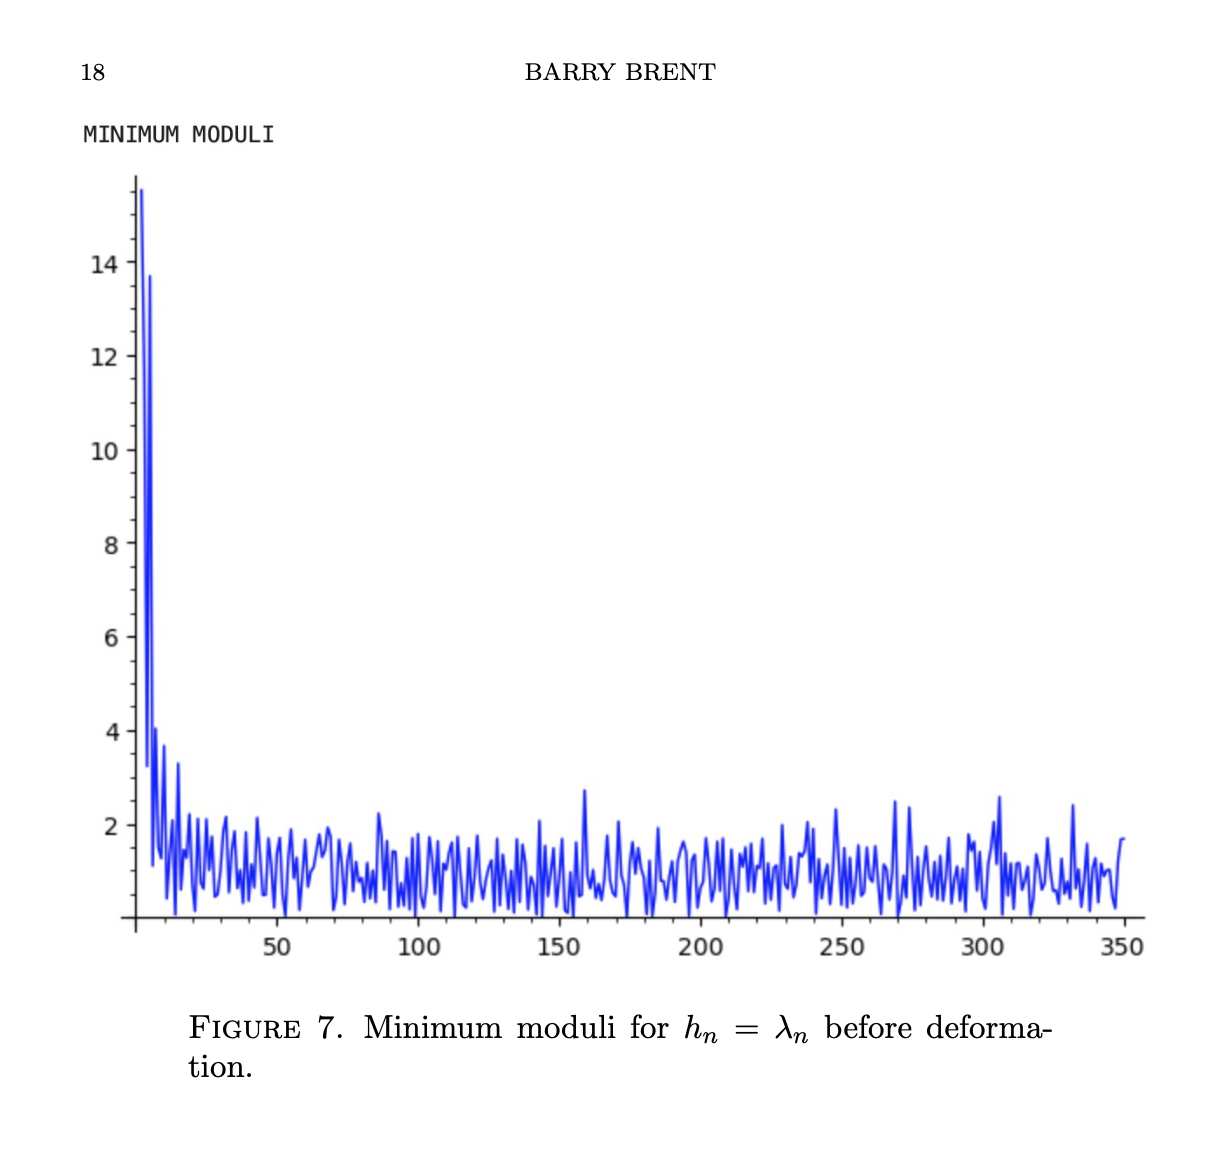
\includegraphics[width=\textwidth]{fig_undeformed_mu.jpg}
\caption{Undeformed $\mu_n$, $h_n=\lambda_n$ (manuscript Fig.~7): $O(1)$, ragged,
near $0$.}
\label{fig:undef-mu}
\end{subfigure}\hfill
\begin{subfigure}{0.49\textwidth}
\centering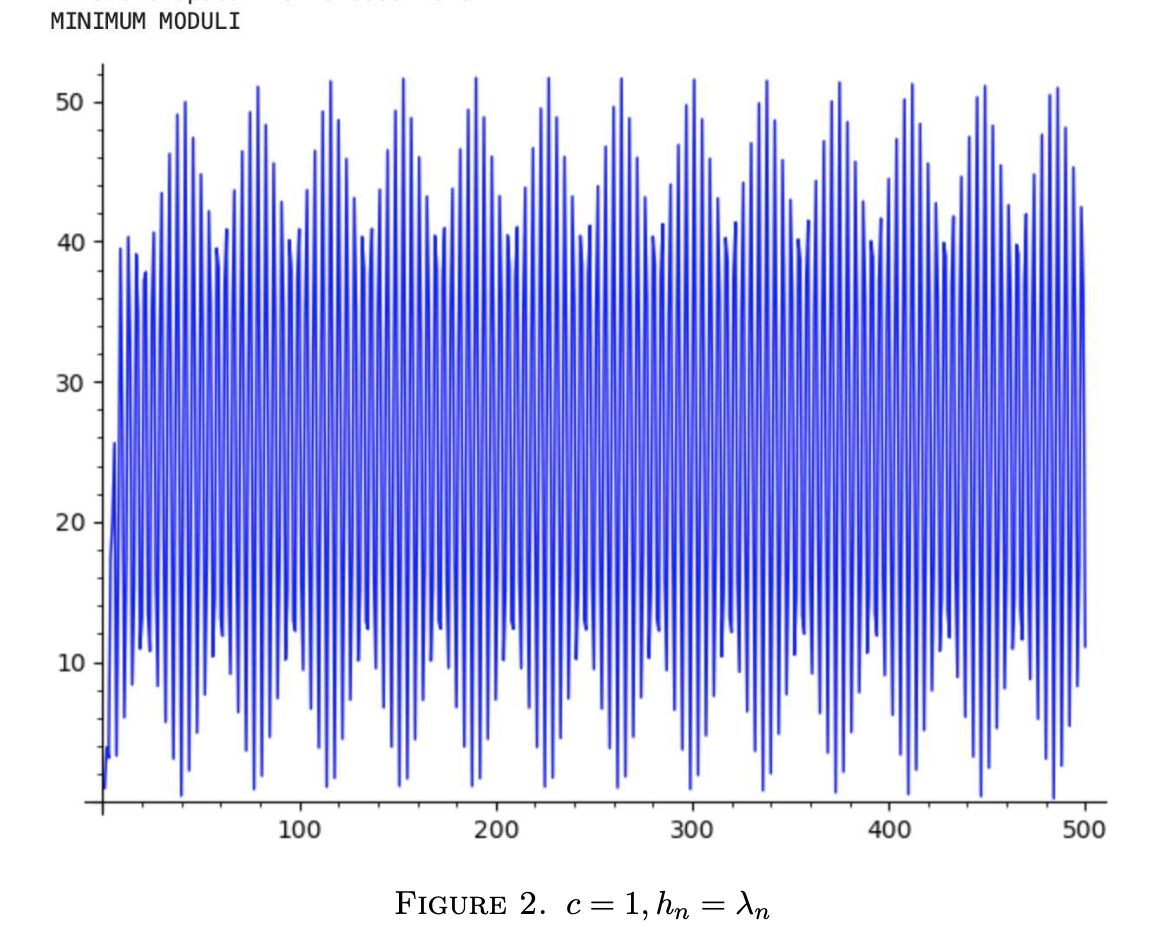
\includegraphics[width=\textwidth]{fig_deformed_mu.jpg}
\caption{Deformed $\mu_n$, $c=1$, $h_n=\lambda_n$ (manuscript Fig.~2): large, regular
oscillation.}
\label{fig:def-mu}
\end{subfigure}
\caption{The same sequence $h_n=\tau(p_n)$, undeformed and deformed. The transformation is
not a translation.}
\label{fig:both-mu}
\end{figure}

\section{Three generating functions, not two}\label{sec:three}

All three characteristic polynomials of \S\ref{sec:setup} are collected by the same kind of
exponential generating function, $\sum_n\chi_n(x)\,t^n/n!=F(-t)\,e^{xt}$, with three
\emph{different} power series $F$ in the role of $H$.

\paragraph{Undeformed.}
Since $J=t\,\tfrac{d}{dt}\log H$, the undeformed generating function satisfies
$\tfrac{d}{dt}\log H = J/t$, so
\[
\log H(t)=\int_0^t\frac{J(s)}{s}\,ds=\sum_{r\ge1}\frac{j_r}{r}\,t^r,
\qquad
\sum_{n\ge0}\chi_n(x)\,\frac{t^n}{n!}=H(-t)\,e^{xt}.
\]

\paragraph{Deformed family.}
Prepending $c$ to the data sequence gives $\tfrac{d}{dt}\log H^{(c)}=c+J(t)$, hence
$\log H^{(c)}(t)=ct+\int_0^t J(s)\,ds$, that is
\[
H^{(c)}(t)=e^{ct}\,G(t),\qquad\text{where}\qquad
G(t):=\exp\!\int_0^t J(s)\,ds=\exp\!\Big(\sum_{r\ge1}\frac{j_r}{r+1}\,t^{r+1}\Big)
\]
is independent of $c$. Let $\Phi_n$ be the polynomials of the $c=0$ deformation, i.e.\ those
collected by $\sum_n\Phi_n(x)\,t^n/n!=G(-t)\,e^{xt}$ (equivalently, the sum of \S\ref{sec:setup}
with the coefficients $g_r$ of $G$ in place of $h_r$). The deformation factor then acts by a
pure shift: substituting $t\mapsto -t$ turns $e^{ct}$ into $e^{-ct}$, so
\[
\sum_{n\ge0}\chi_n^{(c)}(x)\,\frac{t^n}{n!}
=H^{(c)}(-t)\,e^{xt}
=e^{-ct}G(-t)\,e^{xt}
=G(-t)\,e^{(x-c)t}
=\sum_{n\ge0}\Phi_n(x-c)\,\frac{t^n}{n!}.
\]
Matching coefficients of $t^n/n!$ gives the polynomial identity
\[
\chi_n^{(c)}(x)=\Phi_n(x-c).
\]
Thus $G$ is the generating function of the deformed family at $c=0$, and $\Phi_n=\chi_n^{(0)}$.

\medskip

The two backbones $H$ and $G$ share the data $J$ but integrate it differently --- $G$
integrates $J$, while $H$ integrates $J/s$; equivalently
\[
\frac{G'}{G}=J=t\,\frac{H'}{H}.
\]
So $G$ is \emph{not} $H$ multiplied by anything: it is a different analytic function. The
deformation does two separate things, and only the second is a shift:
\begin{enumerate}
\item[(1)] \emph{Prepending} (even prepending $0$) replaces the generating function $H$ by
$G$. This is the structural change, and it is the whole of the visual story.
\item[(2)] The prepended \emph{value} $c$ then rigidly translates the resulting spectrum, by
the identity $\chi_n^{(c)}(x)=\Phi_n(x-c)$: $\spec\chi_n^{(c)}=c+\spec\Phi_n$, whence
\[
\mu_n^{(c)}=\dist\!\big(-c,\ \spec\Phi_n\big).
\]
\end{enumerate}
The earlier ``rigid translation by $c$'' described only step~(2) and silently omitted
step~(1).

\medskip

The two backbones $H$ and $G$ share the data $J$ but integrate it differently --- $G$
integrates $J$, while $H$ integrates $J/s$; equivalently
\[
\frac{G'}{G}=J=t\,\frac{H'}{H}.
\]
So $G$ is \emph{not} $H$ multiplied by anything: it is a different analytic function. The
deformation does two separate things, and only the second is a shift:
\begin{enumerate}
\item[(1)] \emph{Prepending} (even prepending $0$) replaces the generating function $H$ by
$G$. This is the structural change, and it is the whole of the visual story.
\item[(2)] The prepended \emph{value} $c$ then rigidly translates the resulting spectrum:
$\spec\chi_n^{(c)}=c+\spec\Phi_n$, whence
\[
\mu_n^{(c)}=\dist\!\big(-c,\ \spec\Phi_n\big).
\]
\end{enumerate}
The earlier ``rigid translation by $c$'' described only step~(2) and silently omitted
step~(1).

\section{What the change \texorpdfstring{$H\to G$}{H to G} does to the spectrum}\label{sec:change}

The two backbones produce qualitatively different eigenvalue clouds. For $\tau$ at $n=30$
(Figure~\ref{fig:clouds}):
\begin{center}
\begin{tabular}{lcc}
\toprule
 & $\min|x|$ & $\max|x|$\\
\midrule
undeformed $\chi_{30}$ & $1.00$ & $672.9$\\
deformed $c=0$, $\Phi_{30}$ & $42.5$ & $429.1$\\
deformed $c=1$ & $43.5$ & $428.3$\\
\bottomrule
\end{tabular}
\end{center}
and the $c=1$ roots are exactly the $c=0$ roots shifted by $1$ (difference $0$ to the last
digit). In words:

\begin{itemize}
\item \emph{Undeformed} (Figure~\ref{fig:clouds}, left): the roots \textbf{crowd the
origin} --- a dense knot inside $|x|\lesssim50$ with a few far outliers, $\min|x|=1.00$. The
smallest root sits essentially on $0$ and jitters with $n$, so the undeformed plot is
ragged and hugs small values, occasionally diving toward $0$.
\item \emph{Deformed} (Figure~\ref{fig:clouds}, right): the roots lie on a clean
\textbf{ring around an empty central disc} of radius $\approx42$; $\min|x|=42.5$, and there
are no eigenvalues near the origin. The $c=1$ points (orange) sit invisibly on top of the
$c=0$ points (blue): a shift by $1$ is nothing against a radius of $40$.
\end{itemize}

\begin{figure}[H]
\centering
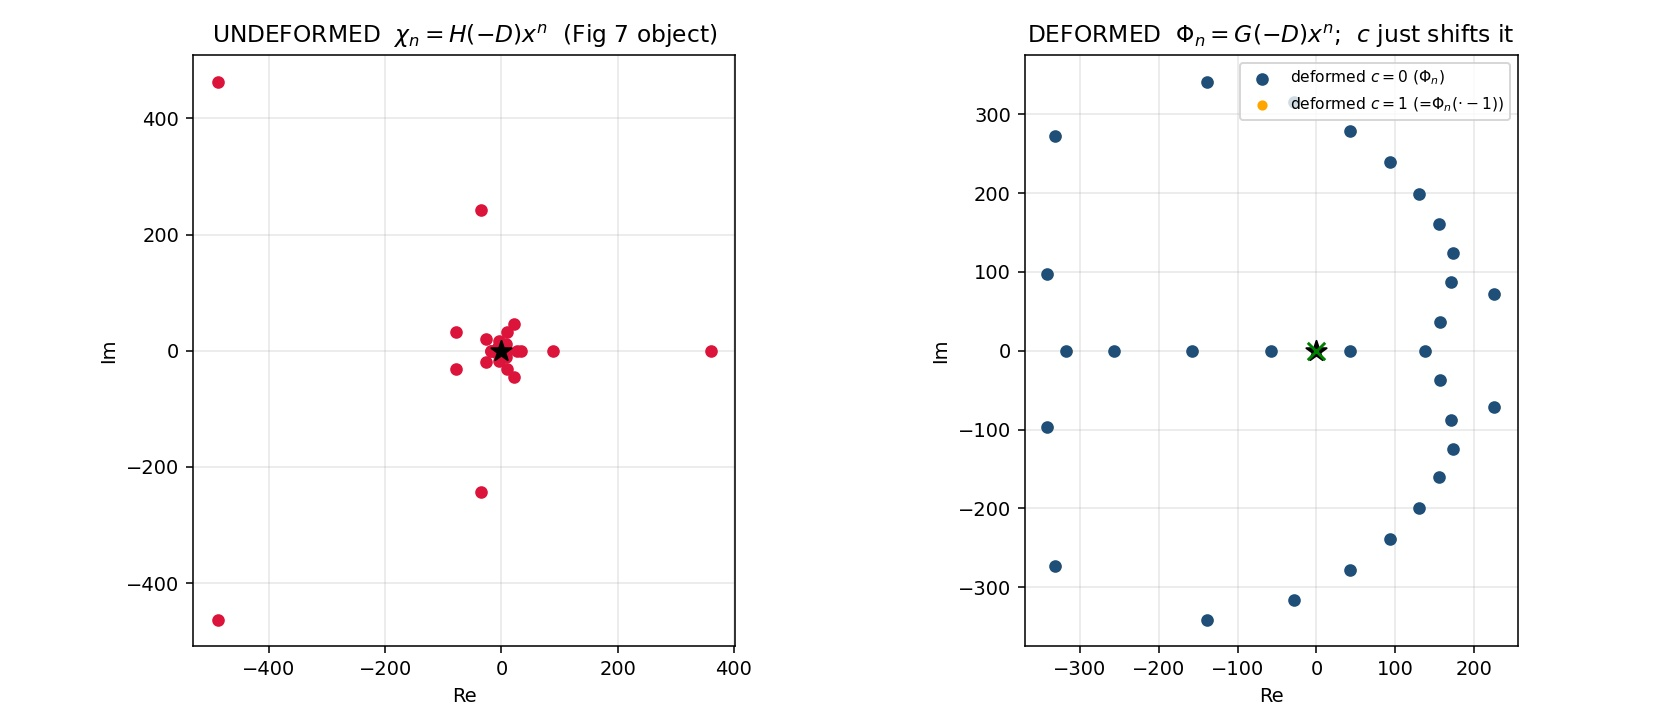
\includegraphics[width=\textwidth]{tau_spectra.jpg}
\caption{Root clouds for $h_n=\tau(p_n)$ at $n=30$. \emph{Left:} the undeformed spectrum
crowds the origin ($\star$), giving a small, ragged $\mu_n$. \emph{Right:} the deformed
backbone $G$ opens an empty disc of radius $\approx42$ around the origin and arranges the
spectrum on a ring; the deformation value $c$ ($-c$ marked $\times$) merely shifts this
ring, so $c=0$ (blue) and $c=1$ (orange) coincide on this scale.}
\label{fig:clouds}
\end{figure}

So the leap from Figure~\ref{fig:undef-mu} to Figure~\ref{fig:def-mu} is the opening of that
empty disc --- the $H\to G$ change of step~(1) --- not the shift of step~(2). The regular
oscillation in Figure~\ref{fig:def-mu}, between $\approx0$ and $\approx50$, is then the
\textbf{inner edge of the ring breathing in and out as $n$ advances}: at some $n$ a root of
$\Phi_n$ swings in close to $-c$, so $\mu_n^{(c)}=\dist(-c,\spec\Phi_n)$ drops toward $0$;
at others the inner edge holds out near $\approx50$. The shift by $c$ only moves the ring's
centre from $0$ to $-c$, a sub-unit nudge here.

\section{The honest boundary, and a probe}\label{sec:open}

\emph{That} the deformation replaces $H$ by $G=\exp\int J$ and opens this ring is exact and
general, and is now visible. \emph{Why} $G$'s spectrum forms a clean, regularly-breathing
ring while $H$'s crowds the origin --- and what sets the oscillation's period and envelope
--- is precisely the question the manuscript leaves open. This note does not claim a theorem
there. What it does is sharpen the question: the phenomenon lives entirely in the analytic
difference between
\[
G(t)=\exp\!\int_0^t J(s)\,ds
\qquad\text{and}\qquad
H(t)=\exp\!\int_0^t \frac{J(s)}{s}\,ds,
\]
specifically in whatever singularity structure of $G$ governs the inner radius of its
spectral ring.

A concrete next probe, at the modest $n$ where the characteristic polynomials are still
well conditioned: track the inner radius of $\spec\Phi_n$ and the angular position of the
root nearest $-c$ as functions of $n$, and test whether the breathing period and the
envelope can be read off the coefficient growth of $G$. (At larger $n$ the same
fixed-precision root-finding wall discussed elsewhere applies, so the inner edge must be
found by a targeted method rather than by computing all roots.)

\begin{remark}[why the deformed plateaus are trustworthy]
The eigenvalues on the ring are $O(\text{radius})$ and well separated, hence well
conditioned, so finite precision resolves them; it is only a tightly clustered, receding
component that is ill conditioned. The deformed oscillations and their envelopes are
therefore real features, not numerical artifacts --- in contrast to the undeformed
$h=2$ plateau analysed separately.
\end{remark}

\end{document}
